% using Elseveir template per https://www.elsevier.com/authors/author-schemas/latex-instructions
\documentclass[review]{elsarticle}

\usepackage{amsmath}
\usepackage{lineno,hyperref}
\usepackage{booktabs}
\usepackage{hyperref}
\usepackage{siunitx}
\usepackage{tabularx}
\usepackage{threeparttable}  
\usepackage{tikz}

\bibliographystyle{elsarticle-num}
% \journal{Journal of \LaTeX\ Templates}
\modulolinenumbers[5]
\usetikzlibrary{calc,matrix}

\begin{document}

\begin{frontmatter}

    \title{
        Conformity and Soft Skills as Determinants of Alternatively Credentialed Non-College Graduate Hireability
    }

    \author[mymainaddress]{John Vandivier}
    \address[mymainaddress]{4400 University Dr, Fairfax, VA 22030}
    \ead{jvandivi@masonlive.gmu.edu}

    \begin{abstract}
        % % Applied Economics author guidelines
        % % https://www.tandfonline.com/action/authorSubmission?show=instructions&journalCode=raec20#words
        % % Should contain an unstructured abstract of 200 words.
        % %   - exactly??? looking at top 3 articles in current issue, #44, abstract varies 172-212
        % %   - am treating 200 as a limit
        % % Graphical abstract / video abstract optional
        % % accepted ref paper (3) stats:
        % % Announcement effects in the cryptocurrency market
        % % abstract len = 172, pages = 15, word count (w extra intro page; overestimate ~100-200 words...plus some long tables...9893)
        % %
        % % Unconventional monetary policy and inequality: is Japan unique?
        % % abstract len = 192, pages = 12, word count (w extra intro page; overestimate ~100-200 words...7397)
        % %
        % % Market competition and corporate performance: empirical evidence from China listed banks with financial monopoly aspect
        % % abstract len = 212, pages = 12, word count (w extra intro page; overestimate ~100-200 words...7856)
        % %
        % % note - Announcement effects in the cryptocurrency market has acknowledgements and disclosure in paper
        % %
        % % el author guidelines: https://www.elsevier.com/journals/economics-letters/0165-1765/guide-for-authors
        % % heswbl author guidelines: https://www.emeraldgrouppublishing.com/journal/heswbl#author-guidelines
        % % While you are welcome to submit a PDF of the document alongside the Word file, PDFs alone are not acceptable.
        % % LaTeX files can also be used but only if an accompanying PDF document is provided. Acceptable figure file types are listed further below.
        % % Articles should be between 5000  and 7000 words in length. This includes all text, for example, the structured abstract, references, all text in tables, and figures and appendices. 
        % % Please allow 280 words for each figure or table.
        Despite targeting technical skills,
        vocational school graduates earn less than college graduates.
        This paper hypothesizes that conformity selection and a perceived deficit in soft skills substantially explain reduced alternatively credentialed non-college graduate (ACNG) hireability.
        % % This paper explores an original data set
        % % to understand the influence of employer skill gap perception on the demand for labor.
        % % Original survey data is investigated to 
        % % Specifically, this study tests the hypothesis that nonconformity stigma is a key factor of reduced hireability for an alternatively credentialed non-college graduate (ACNG).
        % % Results from an original survey in the United States indicates that willingness to break rules is a key factor of hireability,
        % % Results from an original questionnaire administered in the United States indicates that willingness to break rules is a key factor of hireability,
        % % cool, concise words :D https://en.wikipedia.org/wiki/Microdata_(statistics)
        Microdata from the United States confirm a perceived soft skill deficit for ACNG labor.
        Results indicate that conformity is a critical factor of hireability,
        but the direction of effect is heterogenous by employer type.
        % This analysis demonstrates the importance of perceived skill gaps and conformity selection when compared to other widely recognized factors of hireability.
        Conformity and perceived skill gaps explain about one-third of hireability variance.
        % Perceived soft skill gaps demonstrate importance by explaining about as much variance in hireability as the sum of the effects from state of residence and industry of occupation.
        % Perceived soft skill gaps explain about as much as the sum of the effects from the state of residence and industry of occupation.
        Perceived soft skill explains more hireability variance than widely recognized factors like the industry of occupation.
        Opposite conventional explanation, results suggest that conformity reduces hireability on average.
        % Respondents tend to perceive ACNG candidates as creative types and an even mix of high and low performers.
        Respondents tend to perceive ACNG candidates as an even mix of high and low performers.
        % ACNG job candidates tend to be perceived as creative types and an even mix of high and low performers.
        % % the risk aversion explanation subsumes the explanation from positive conformity selection, but incentives for negative conformity selection remain.
        % % that is, conformity is not a direct production function input, but it is a signal of low labor productivity variance.
        % % risk aversion explains why employers would prefer less variance regardless of the average comparative productivity estimate.
        % Employer risk aversion toward labor productivity contributes to the explanation of low ACNG demand.
        Evidence favors employer risk aversion toward labor productivity as a preferred explanation of low ACNG demand.
        ACNG labor is perceived as low in conscientiousness and body language communication skills compared to college graduates.
        % Evidence favors an explanation of low demand for ACNG labor
        % % compared to the recent college graduate 
        % based on risk aversion over positive conformity selection.
        %
        % % it's all about that body language skill!
        % % This analysis shows that perceived skill gaps provide more statistical explanation of hireability than
        % % Perceived skill gaps are more important than widely recognized factors of hireability including industrial and state effects.
        % % Soft skills are particularly important.
        % The skill of communication using body language is perceived as a key comparative advantage of recent college graduates over ACNG job candidates.
        % % Recent college graduates and ACNG job candidates share many of the same perceived skill gaps...
        % % in paper, discuss: sum rulebreaker_ideal rulebreaker_ngwac rulebreaker_recentcollegegraduat rulebreaker_typicalemployeeatmyc
        % The conclusion incorporates discussion of public misperception on the cost of vocational school and suggests that nontraditional postsecondary education is undervalued in the United States.
        The conclusion incorporates discussion of public misperception on vocational school costs and suggests activities to reduce unconscious bias.
        % % Results collectively indicate that nontraditional postsecondary education is more valuable than would be expected in the absence of such results.
        % % Marginally increased social demand would be socially beneficial.
    \end{abstract}

    \begin{keyword}
        education economics, signaling, hireability, conformity, vocational               %%% not grammatical
        \MSC[2010] I20, I21, J23, J24                                                     %%% not grammatical
    \end{keyword}

\end{frontmatter}

\pagebreak
\linenumbers

\section{Introduction}

% Some optional TODO:
% . talk a bit more about state and industry and see if we can draw a pattern out (STEM industry? high-pop / Democrat states?)
% . `...and employment in the information technology industry yields a positive coefficient`: give beta and sd
% . use table since there are 3 cases of beta and sd (potential TODO: long paper food...2 additional tables; also a summary stats table; perhaps also a diagram)
% . if allowed, another diagram to aid the model section and make the theory clear;

% MB protip: intro outline follows:
% --hook or tension
% --where we are now
% --the importance of your question
% --preview of results

A substantial gap exists between the skills expected by employers and those possessed by college graduates\cite{mcgarry2016examination, malik2017great, abbasi2018analysis, gingras2000there}.
Experts view college alternatives,
including vocational school,
to be useful for technical training,
but the traditional college degree retains a wage premium over vocational education.
Unemployment, underemployment, and other adverse labor outcomes follow a similar pattern\cite{smith_2011}.
This paper seeks to resolve the apparent discrepancy between these outcomes while preserving the mainline economic view that employers pay for perceived job candidate skill.
% or expected marginal revenue product of labor
To explain the apparent discrepancy,
this paper tests the hypothesis that employers expect an offsetting non-technical skill deficit when considering an alternatively credentialed non-college graduate (ACNG).
I find evidence that employers and the general population in the United States expect a low level of soft skills from ACNG job candidates.

Alternative credentials refer to credentials other than the undergraduate degree\cite{brown2017complex}.
The category includes, for example,
industry certifications,
portfolios of work,
% transcripts of accredited or unaccredited course work,
digital badges, and other records of unaccredited learning and achievement.
Individuals pursuing alternative credentials typically intend to leverage it toward better employment.
That is, they typically have the same goals as a college student.
Many individuals obtain alternative credentials as a supplement to the college degree.
Such a situation is Pareto-superior to degree attainment alone and is therefore intentionally excluded from the analysis.
This paper focuses on the comparatively interesting case of alternative credentials as a substitute for the college degree to diagnose comparative disadvantage at the skill level.
If a specific skill set explains labor outcome differences, alternative learning providers can improve their products to reduce the outcome gap.
% as opposed to the case where no known skills explain the gap and it's just a label stigma

% Alternative credentials can be obtained quickly and cheaply relative to college.
% Obtaining a college degree signals intelligence, conscientiousness, and conformity,
% but it may not signal technical skill\cite{horton_2020}.
% Alternative credentials signal technical skill.
% As such, they provide an effective supplement to the college degree.

% This paper is concerned with another use case in which the college degree is entirely substituted.
% In that situation, employers may apply a noncollege stigma.
% This is particularly the case for roles which are typically occupied by degree holders.
% Noncollege stigma is a presumption, expectation, or bias toward perception of a skill gap of a certain kind.
% Whether the gap exists in fact is out of the scope of the present paper.

% Technical skill generally implies intelligence.
% Alternative credentials, then, fail to signal two qualities compared to the college degree.
% Alternative credentials fail to signal conscientiousness and conformity.
% Interestingly, some employers may demand some level of nonconformity.
% Employers may also presume a certain lack of soft skill on the part of highly technical applicants.
% % Finally, employers may use alternative credentials as a proxy for other employee characteristics like income, education, race, and gender.

% % a missing link for future research: hireability only correlates with actual hiring decisions it isn't a hiring decision
% Hiring decisions reflect boundedly rational demand for skilled labor.
% The college degree and alternative credentials provide two qualitatively distinct signals of skilled labor.
% The hireability of individuals in possession of these credentials has been studied,
% but the underlying determinants are not clear.
% This paper hypothesizes that perceived skill gaps are important determinants of hireability.
% This paper further hypothesizes that perceived skill gaps are qualitatively different between college graduates and others.
% % In particular, this paper hypothesizes that a noncollege stigma is obtained for candidates without a degree in pursuit of roles typically filled by degree holders.
% % soft skill bias in particular

% three interesting follow-on questions:
%   1. do employers have such a bias
%   2. is such a soft skills gap presumption actually true
%   3. if true, due employers overvalue the soft skills gap
% related paradox: most people won't be in a job for 4-5 years,
% so why do they need to show conscientiousness and conformity towards the 4-5 year bachelor's goal line?
% hard skill stigma: in my experience, people who are highly technical are hard to work with
% soft skill bias: I am favorable bc i think u have soft skills (and maybe this is efficient...enter eq/iq discussion)

% This paper tests the hypothesis that there is a lack of hireability an ACNG (ACNG) is explained by an offsetting perceived lack in non-technical skills.
% In particular, this paper hypothesizes that ACNGs are seen as nonconformist and lacking in soft skills or non-technical skills.
% These deficits explain why an ACNG would not be a preferred source of labor in many cases,
% even if such a candidate does possess superior technical skill.

% technical skill has negative coefficient but magnitude and reliability (p-value/variance) are weaker; overall, less important effect
% hypothesis stems from signaling model.
% This paper proposes skill gaps are perceived in particular among soft skills for alternatively educated individuals.
% one might argue employers are mistaken here; technical work may involve higher, not lower, conscientiousness; ya maybe but out of scope.
% that is, we test social stigma and skill-level / decomposed stigma; an application of the signlaing model.

% Experts view college alternatives including vocational school as useful for technical training, but the traditional college degree retains a wage premium over vocational education.
% This paper hypothesizes that employers pay for skill.
% As a result, lower wages for technically skilled individuals are hypothesized to derive from an offsetting perception of skill deficit elsewhere.
% That is, this paper hypothesizes that employers view an ACNGs (ACNG) as lacking in soft skills.
% This paper hypothesizes that employers expect a skill deficit, although not a technical skill deficit, 
% This expected deficit explains the variance in labor outcomes.

% Sustained rising costs to higher education motivate periodic review of the return to the college degree.
% Despite rising costs, Americans have become more educated than expected over the past decade.
% Trades have contemporaneously seen a labor shortage.

% actually, trade school enrollment is increasing faster than undergraduate enrollment
% https://www.chronicle.com/newsletter/the-edge/2020-01-22
% By 2020, They Said, 2 Out of 3 Jobs Would Need More Than a High-School Diploma. Were They Right?
% overinvestment in college seems to cause a technical labor shortage, but the market is compensating by enrolling more technical folks too
% https://www.theatlantic.com/education/archive/2019/03/choosing-trade-school-over-college/584275/
% undergraduate enrollment has slowed recently and many employers have dropped the college degree requirement
% https://www.npr.org/2019/12/16/787909495/fewer-students-are-going-to-college-heres-why-that-matters
% it is not the case that employers are increasingly demanding the college degree, but it is the case that many do today. Let's examine their reasons.
% peak college?

% An undergraduate degree is a historically reputable investment.
The signaling model has become one of the two standard explanations of the value of the college degree.
Signaling theory provides three advantages over human capital theory for the present study.
First, signaling theory can explain labor outcome variance when human capital is held constant.
% First, signaling theory is able to explain labor outcome variance across labor types when skills are totally equal.
% Under a human capital model, in contrast, a variety of labor outcomes would directly imply variance among input labor.
% The present paper expects that skills for the ACNG compared to other labor types are not totally equal, but this must emerge as a result rather than a presumption.

Second, the signaling model empowers a questionnaire research design.
In an idealized human capital model, the measures of human capital would correspond to production process inputs.
To establish a wide array of such skill measures would be complicated and prone to measurement sensitivities, assumptions, and errors of various kinds.
In this framework, a questionnaire is a second-best design that provides a proxy for the functional measure of skill.
Signaling theory takes the reverse approach.
According to the signaling model, employer perception and evaluation drive their willingness to pay for a job candidate.
The manner is in which employer perception relates to job candidate technical skill, if at all, is secondary.
In this framework, a questionnaire is ideal.
% In this framework, a questionnaire is a direct measure of the functional construct, which is the opinion of the employer.
An additional benefit of using a questionnaire is the ability to ask hypothetical questions.
In pondering hypotheticals,
employer evaluation of a credential or signal can be isolated from the human capital variance,
which occurs in actual job candidates.

Third, signaling theorists have laid out a testable hypothesis for weak labor outcomes among non-college graduates.
Following this model, scholars claim that the college degree signals intelligence, conscientiousness, and conformity\cite{caplan2018case}.
% Since immediate college enrollment is the normal course of action for high school graduates,
Nontraditional education, in contrast, is hypothesized to signal nonconformity.
Nontraditional courses can be completed in a shorter time and with reduced entry qualifications relative to the traditional degree.
For this reason, alternative credentials hypothetically signal low conscientiousness relative to the college degree.

% Proponents of the signaling model often prefer employer-oriented explanations of college enrollment.
% In this explanation, employers prefer college graduates because the college degree signals intelligence, conscientiousness, and conformity.
% While a technical credential signals intelligence and technical skill, the absence of a degree yields a perceived gap in the mind of the employer.
% There is a perceived comparative lack on the part of the non-college graduate with respect to conscientiousness and conformity.
% This paper tests this hypothesis.

% An agent-based explanation would be that high school graduates are not taught about these alternatives.
% The college degree is popular, has a well-defined return, and is low in risk.
% Particular alternative programs are obscure and often lack a well-defined return.

% Other research indicates that conscientiousness and conformity are not always desirable labor qualities.
% There is some reason to doubt the hypothesis that lower perceived value is attributable to signaling differences in conscientiousness and conformity.
% Research indicates that extreme values for either factor in either direction may be detrimental to productivity.

% TODO: long paper food...uncomment below section as it implies we should be doing marginal analysis. Then do marginal analysis, and K*K skill interactions
% TODO: maybe move to results section when we talk about conscientiousness
% Research indicates a goldilocks level or bliss point for both conscientiousness and conformity is likely to exist.
Research indicates that employer demand for employee conscientiousness and conformity follows a bliss point pattern.
Excess individual conscientiousness can disturb team performance\cite{curcseu2019personality}.
Conformity can lead to a lack of innovation and suboptimal organizational practices\cite{symon2006neglected}.
% Psychologists also state that
Conformity selection occurs in part through heuristic rather than deliberate cognition.

% Because a single measure operationalizes each of these effects and their own negation, a fixed sample size is relatively unlikely to identify an important coefficient.
% Because these factors are sometimes demanded and in other cases the inverse is demanded, a factor coefficient may be harder to identify and may only represent the average effect, even if the average effect is hardly predominant in practice.

% The psychological problem is related to but distinct from the pure logical problem that a totally conformed mind is necessarily incapable of innovation.
% Firm innovation requires an underlying capacity for individual innovation.
% Firms must have some capacity for innovation to sustain profit in a growing economy.
% Even if conformity selection is a correct explanation of ACNG aversion, then, it may not be an ideal practice when viewed through the lense of technical or economic efficiency.
% Risk aversion is compatible with a sometimes-concious, sometimes-heuristic decisioning model.

% Innovators, leaders, and high-performers are three kinds of virtuously nonconformant labor.
% Because conformity is sometimes undesirable and sometimes desirable,
% the effect may neutralize itself in an ordinary OLS stastistical analysis.
% The effect may not be identified as important or significant in any particular direction.

Risk aversion is a distinct explanation for conformity selection.
Some employers are not able to evaluate an alternative credential with confidence.
Such an employer views ACNG labor as a gamble with some odds of positive or negative outlier value.
The employer may not prefer to hire such a candidate due to risk aversion,
even if their point estimate for ACNG labor value is higher than their point estimate for a recent college graduate.
If firm size effects are positively associated with ACNG hireability, this will add weight to an explanation based on risk aversion.
% Reasons for this include: 1) failure to deliver can be catastrophic, so low performers may be disproportionately untolerable.
% Revenue consistency, timeline, reputation, quantity produced targeting, large min skill labor cost and marginally small pay increase to achieve adequate production.
% Performance monitoring and turnover costs reinforce this
% zb states I'm assuming constant cost per hire...actually I allow that some portion of large-firm hireability is due to better ability to distinguish low vs high
% other than that effect, the remainder would be attributable to risk aversion.
% yes, the null hypothesis is no difference in cost per hire; but I can also support that which I suspect...turnover costs are proportionally smaller for large firms
% these firms are able to specialize and economize in hiring, plus they are more likely to have high-skill candidates that can better interview and recruitment tech+processes that scales
% TODO: long paper food... consider below articles and flesh out the risk aversion to firm size interaction thing
% note turnover cost calculation is complex but we proxy of just cost to hire. A + B below support cheaper for large firms. (C reinforces B)
%   A) "As stated in a study by the National Association of Colleges and Employers, hiring an employee in a company with 0-500 people costs an average of $7,645."
%   B) "Another study by the Society for Human Resource Management states that the average cost to hire an employee is $4,129, with around 42 days to fill a position."
%   C) "According to Glassdoor, the average company in the United States spends about $4,000 to hire a new employee, taking up to 52 days to fill a position."
% related but doesn't solve the issue: https://builtin.com/recruiting/cost-of-turnover
% https://toggl.com/blog/cost-of-hiring-an-employee
% The highest performing employers, however, will be able to distinguish desirable from undesirable candidates within the unconventional pool.
% Risk aversion varies naturally among firms. <- probably don't write this line in paper as a reviewer can always posit there is a further reason you are missing
% Some employers that are high in risk aversion will provide a net preference to ACNG due to nonconformity preference.

% TODO: long paper food...below section is part of intro or perhaps model...
% \subsection{Process Explanations of Suboptimal Wages}

% Basic price theory holds that an employer should pay wages equal to the marginal revenue product of labor.
% In the real world, measuring candidate productivity at hiring time is costly and imperfect.
% % This produces a technical error which assumes alignment between the goals of the firm and a hiring team.
% A further issue is identified when the hiring team is scrutinized for principal-agent problems.
% The hiring team is composed of individuals with preferences, calculative limitations, and other biases.
% Monitoring and correcting for these problems is expensive,
% so firms will heterogenously realize some aggregation of these individual definiciencies.

% Exacerbating the already necessarily imperfect hiring process are candidate-side problems.
% Firms must hire among a finite, potentially small, number of candidates.
% Risk aversion to time expense and other search costs may lead a firm to approve a suboptimal candidate\cite{simon1976substantive}.
% In some cases, candidate pools may be systematically problematic.
% In law and medicine, for example, extensive education and training are legally required.
% These policies further restrict the candidate pool, inflate expected wages, and systematically alter the content of education in a politically-motivated manner.
% Market forces implement hiring as a lumpy expenditure process to begin with, but certification requirements, wage regulation, and other policies extend the problem.

% The prior discussion highlights many locations of hiring process inefficiency.
% The practical importance of magnitudes and kinds of such effects are described in a legion of related papers.
% A meager sampling of five such effects would include the attractiveness effect and many other issues related to gender bias\cite{quereshi1986physical},
% agentic behavioral stigma\cite{steffens2009feminization},
% and complex biases related to communication style\cite{brouer2017gender, nijs2019effects, sampugnaro1983nonverbal}.
% Sung et al find that impression management meaningfully weakens disability stigma\cite{sung2017disclose}.
% These tactics are transferable in part to noncollege stigma mitigation.
% Finally, there are a wealth of concerns about the effects of social media.
% For one, it presents a channel for the revival of religious discrimination\cite{esposito2018signaling}.

% In the face of so many important inefficiencies, one begins to wonder whether the original theory holds any water at all.
% Papers which identify matching effects, including the present paper,
% serve to limit the proportion of explanation attributable to bias and redeem the elementary price theory story to some extent.
% Prior work demonstrates the important of matching effects in the form of norm compliance\cite{francesco1981gender}.
% Meta-accuracy is a kind of matching measure, and it has been shown to move positively with hireability\cite{renier2018no}.

% \section{Literature Review}
% TODO: long paper food...lit review exists in Announcement effects in the cryptocurrency market
% TODO: long paper food...expand on the signaling model vs the human capital model
% Faster and cheaper alternatives to college exist, but high schools prefer immediate college enrollment over alternative options at a rate of nearly 2:1.
% A New U: Faster + Cheaper Alternatives to College
% Faster and cheaper alternatives to college exist, but the typical student prefers to immediately enroll in college.
% Five student-oriented explanations include an inflated perception of the return to college,
% lack of awareness about alternative programs,
% social pressure to pursue college over alternatives,
% inability to confidently compare returns to alternatives,
% and risk aversion which favors college as a low-risk option despite high cost.


\section{Data and Methodology}
% note: description of data / model / methodology: one section in a short paper; can be broken into seperate sections for a long paper...or can it? seems kinda intertwined
% for this paper: methodology [i. model / method of analysis, ii. description of data collection iii. additional description of data as needed at factor level]
% I don't feel the need to spell out an OLS model equation unless requested by a reviewer
% I don't feel the need to spell out the risk aversion model equation unless requested by a reviewer (it's just a signal multiplier on actual skill which varies by credential and employer)
% the risk aversion model i feel is more interesting, but it would be an inappropriately high level of focus and detail for an item of secondary interest

% The method of this study begins with a decomposition of the main hypothesis into three simple statistical tests.
% This study applies the three-step method to the case of the ACNG, but the three-step method itself is sufficiently general to apply to any measurably distinct job candidate type.
% First, skill gaps are identified as independent factors with a general ability to explain hireability.
% Second, the coefficient for a
% Finally, gaps in soft skills are hypothesized to be more important than technical skill gaps.
% If the above three conditions hold, ACNG labor dispreference can be explained with or without comparing labor outcomes to the college graduate.

A simple model of demand for labor provides context for the hypothesis of interest.
This model is clarified in Equations \ref{eq1} and \ref{eq2}:

\begin{subequations}
    \begin{equation}
        % maybe S is not S_j showing S is a non-person-specific credential
        % but I like S_j because it is *those credentials possessed by j* which can be a unique collection + unique work history, other unique signal, etc...
        S_j = f(H_j)
        \label{eq1}
    \end{equation}
    \begin{equation}
        w_{ij} = E_i(MRP_j) = f_i(S_j)
        % alternatively, D_i(L_j) = E_i(MRP_j) = f(S_j, i)
        \label{eq2}
    \end{equation}
\end{subequations}

Job candidate $j$, generates a signal of productivity, $S_j$ from unobserved human capital, $H_j$.
Employer $i$, forms an expectation of the marginal revenue product of $j$ on the basis of $f_i(S_j)$, an employer-specific evaluation of $S_j$.
A specific employer is willing to pay a specific job candidate wages of $w_{ij}$.

This study uses ordinary least squares (OLS) regression analysis to estimate the effect of perceived skill gaps on hireability.
An employer is willing to pay more for a relatively hirable individual.
The representation of willingness to pay makes hireability a proxy of demand for labor and $w_{ij}$.
% measure or proxy? proxy bc diff units.
% this is questionable because hireability is technically the willingness to execute a wage integrated over some expected time period (average employee tenure)
% but then, that integrated wage would just be wage multiplied by some constant and we would need to divide by some constant since hireability is a probability
% so, hireability should correlate directly to wage after all
% you also might say hireability is theoretically closer to an estimate of productivity...but who cares it's once again equal
% and we want to frame the overall model as a simple labor demand model.
%
% Equally, a respondent is making an expected productivity statement when scoring hireability
% This study presumes that employers are willing to pay less for an ACNG.
% This study also presumes that ACNG labor has better technical skill.
This paper hypothesizes that employers preferentially value soft skills in the course of $f_i(S_j)$
to explain the reduced willingness to pay for ACNG labor relative to college graduate labor.
If employers do bias toward soft skills in job candidate evaluation,
one or more soft skills should yield a negative coefficient
% of an economically important magnitude
in a regression on hireability.

% The hypothesis that employers associate soft skill deficiency with ACNG labor is based on a simple model of labor demand.
% As such, the top-level model is a model of demand for labor.
% This is how we derive the hypothesis of offsetting deficiencies from a lower ACNG wage.

This study uses original cross-sectional data from an online self-completed questionnaire ($n = 212$).
The data is available for replication or any other use\footnote{
    See \url{https://osf.io/8qtxf/?view_only=95b0c0b0c65e4b7983198cc87c2ab733}
    for data and statistical analysis code used in this study.
}.
% Responses were submitted using the SurveyMonkey web application.
The Amazon Mechanical Turk crowdsourcing service provided respondents for the questionnaire.
Respondents were United States citizens at or over the age of eighteen,
paid for participation,
and selected on an opt-in, first-come, first-serve basis.
The survey administration took place in July of 2020.
% MAYBE TODO: above paragraph could be moved to after categorical and likert-type discussion
% MAYBE TODO: I could explain that AMT has been shown by my other paper to be bias-free for this right hand param
% and that I purchased 225 samples on the basis of 1) over 100 for large numbers to kick in, and
% 2) experience with the other survey hinted this would be on the lower end of what was needed for significance.

The survey includes 65 questions in two sections\footnote{See Appendix A for a full copy of the survey.}.
The first section captures respondent characteristics,
and the second section captures perceived skill relative to hypothetical job applicants.
Employer responses did not significantly differ from the general population,
so results generally hold for both employers and the United States population.

Regression variables in this study are categorical or Likert-type responses based on a scale from 1 to 10
\footnote{
    It is an accepted practice to treat Likert-type responses as either categorical or continuous for regression analysis.
    % This paper treats such variables as continuous, which is consistent with the theoretical structure of the demand curve and the other variables of analysis.
    % it's also consistent with normalized reporting of real skill measurement; even percentiles themselves are continuous entities.
    % ie, I could do marginal analysis; and i did a little but i'm not talking about it lol.
    Jaccard and Wan provide support for continuous analysis of Likert-type data.
    They note that severe departures from the assumptions on cardinality "do not seem to affect Type I and Type II errors dramatically,"
    particularly when the Likert scale is five or more points\cite{jaccard1996lisrel}.
    This paper uses a 10-point scale and treats these data as continuous.
    A 10-point scale is equivalent to a continuous response from 1 to 10 with rounding.
    %
    % In the current data set, continuous treatment provides a consistent and conservative fit of the data with high confidence.
    % Categorical decomposition yields higher fit with less significance in each category of Likert response.
    % This indicates categorical decomposition may represent a case of overfit and is therefore an additional reason not to prefer that analytical approach.
    %
    % % TODO: long paper food...add marginal fx and u get a third reason Likert as continuous is gtg
    % Finally, treating Likert-type responses as continuous is structurally defensible in this particular study.
    % The notion that Likert-type responses are purely ordinal would make the notion of marginal effect absurd and incalculable,
    % but willingness to pay for labor, conscientiousness, and other factors used in this study are known to exhibit marginal effects in the literature. % TODO: I could cite but it's pretty obv
    % See the results section where a marginal effect from conscientiousness is identified and interpreted in a meaningful way.
    %
    % TODO: but probably not...I could also cite a paper where an economist uses Likert questionnaire data as cardinal
    % i would be happy to use a categorical-like treatment if not for this, and the latter might even have better fit but it could be overfit.
    % finally, an alternative approach would be to treat likert responses as categorical, but the continuous treatment has less fit and more structural justification
    % categorical treatment is a relative overfit
    % likert-type units can be considered direct psychological measures or economic proxies.
    % The likert-type response curve can be thought of as a function of actual skill;
    % b. decent paper on ordinal independent variables: https://www3.nd.edu/~rwilliam/stats3/OrdinalIndependent.pdf
    % c. more on this: https://www.researchgate.net/post/Is_a_Likert-type_scale_ordinal_or_interval_data
}.
Higher Likert-type values indicate greater agreement with a statement that varies by variable.
Categorical variables include state of residence,
the industry of occupation,
employer status,
firm size,
and a measure called duration.

Duration measures the length of time the respondent believes it takes to obtain an alternative credential.
Employer status describes whether an individual makes hiring and firing decisions in the course of their employment.
The variable takes one of three values: yes, no, or unemployed.
Employer effects refer to the case where an individual states that they do make hiring and firing decisions.
State of residence refers to a state within the United States or the District of Columbia.
While it was permitted, no actual responses identified the District of Columbia as a residence.

Regression analysis includes three other factor groups, and they are measured using Likert-type units.
They include hireability, rulebreaker effects, and perceived skill gaps.
Hireability is the dependent factor.
It indicates the degree of agreement that, "For many professions, alternative credentials can qualify a person for an entry-level position."

% The unit of factor coefficients for nonconformists and skill gaps is hireability per Likert-type unit, where hireability is also a Likert-type unit.
% Rulebreaker effects refer to a collection of three factors that describe the way employers think about nonconformists, or "People who are willing to break formal or informal rules and norms."
Rulebreaker effects refer to a collection of three factors that measure respondent agreement with statements about nonconformists, or "People who are willing to break formal or informal rules and norms."
% The three rulebreaker questions measure respondent agreement with statements 
The first statement indicates that nonconformists present a risk to a company's reputation, productivity, or value.
This statement received the least agreement and greatest response variance among three qualitatively different descriptions of nonconformists ($\mu = 6.40, \sigma = 2.55$).

The second statement indicates that nonconformists are held back by rules and "could just as easily be high performers as low performers."
% The second statement indicates that people break rules which hold them back, and that nonconformists "could just as easily be high performers as low performers."
% MAYBE TODO: standard error instead of or in addition to standard deviation. maybe make a table since there are at least three cases of similar report.
This statement received the most agreement and least variance among rulebreaker statements ($\mu = 7.42, \sigma = 1.91$).
The agreement with this statement provides evidence against the thesis that employers value conformity for its own sake.
In turn, this adds weight to the theory that employers value conformity as a risk aversion tactic while knowing that nonconformity signals positive outlier potential.
The third description of nonconformists states that they are creative, innovative, and may benefit company culture ($\mu = 7.25, \sigma = 2.03$).
% managers are wary of ACNG, having high correlation with "Rule Breakers Risky"
% reg _ismanager1 rulebreakersnormsmightbedoingsob rulebreakersnormsprobablyhaveaha rulebreakersnormstendtobegiftedi

% % MAYBE TODO: sentence below can be shortened and we can introduce likert-type unit as distinct from likert-type response since it's a computed value
% Perceived skill gaps are computed from perceived skill questions in the second section of the survey.
% % Respondents do not directly report perceived skill gaps.
% % Instead, responses indicate perceived skill level for particular skill and a particular type of job candidate.
% % 13 skills are analyzed and 4 job candidate types are surveyed, for a total of 52 questions in the second section on perceived skill.
% % MAYBE TODO: citation to "make response anchoring appropriate"
% % Each section begins with a contextual message to normalize response anchoring.
% % Questions are provided in nonrandom order for the same reason.
% % Data from the second section is used to calculate perceived skill gaps.
% For each of 13 skills, the respondent is asked to imagine four types of job candidate.
% One type of candidate is an ideal candidate.
% Raw perceived ACNG skill gaps are calculated by differencing the perceived skill of an ideal candidate with the perceived skill of an ACNG.
% % technically, the actual skill of an ideal candidate equals the perceived skill so the adjective is extraneous; but let's be consistent and not confuse reader.

Perceived skill questions in the second section of the survey allow for two ways to calculate perceived skill gaps.
Perceived skill gaps are measured separately with and without overqualification effects.
Overqualification effects are important in external research\cite{green2007there, raybould2005over}, but skill gap analysis that ignores these effects is also routine\cite{blake_2018}.
% MAYBE TODO: cite more than 1 person who ignores overqualification
% MAYBE TODO: just have one dependent variable and don't mention the other. it's something i did at analysis time, but may be confusing in the paper.
%       alternatively, keep 'em both and call the second a robustness test...that is what i use it for anyway

Perceived skill is a Likert-type response reporting agreement with the statement that a particular candidate has a particular skill.
For each of 13 skills, the respondent imagines and reports skill levels for the ideal candidate,
the average actual employee,
the average recent college graduate,
and the average ACNG.
Raw perceived ACNG skill gaps equal the difference of the perceived skill of an ideal candidate with the perceived skill of an ACNG.
The perceived skill gap with overqualification effects equals the raw perceived skill gap.
The perceived skill gap without overqualification effects is calculated as the raw skill gap or zero if the raw skill gap value is negative.

Rulebreaker effects and perceived skill gaps are structurally linked.
One of the skills that respondents evaluate is nonconformity, or "willingness to break formal or informal rules and norms."
Nonconformity interacts with employer disposition to rulebreaking.
For this reason, discussions on the importance of skill gaps include discussion on rulebreaker effects.

% TODO: long paper food...spell out OLS model. it is hireability = f(employer status, firm size, duration, industry, state, rulebreakers, skill gaps) there is also the skill gap-it interaction...

% MAYBE TODO: delete this paragraph
These methods allow for the identification of a preferred model that explains hireability using perceived ACNG skill gaps.
The identified model will support the hypothesis if soft skills are more important than technical skill gaps. % and negatively affect ACNG hireability.
The model will support the risk aversion explanation of ACNG hireability over an explanation from conformity selection if large employer size is positively associated with hireability.
% If employers preferentially value soft skills then soft skill gaps should be identified as important and negatively relate to ACNG hireability.
% MAYBE TODO: I said this earlier in this same section...am I referencing the main hypothesis too often or is it healthy?
% MAYBE TODO: I also expect signs to be generally negative and soft skills should be statistically significantly less for ACNG compared to recent college graduate
% MAYBE TODO: rulebreaker effects and firm size effects also contribute to solutioning the risk aversion hypothesis

The last section of results goes over comparative results between ACNG skill gaps and gaps among recent college graduates.
The comparative analysis provides additional confidence in the data by replicating the hireability gap between ACNG labor and recent college graduates reported in external research.
Model 6, the initial comparative model, results from an adjustment of Model 5, the preferred noncomparative model of hireability.
Each perceived skill gap in Model 5 is replaced with a comparative skill gap variable to generate Model 6.
Comparative skill gaps equal the perceived skill gap for the ACNG minus the recent college graduate's perceived skill gap.
Multiple regression of these comparison factors on hireability demonstrates which, if any, perceived skill gaps are important distinguishers of the ACNG from the college graduate.
Identification of significant differences with a total negative effect on hireability will replicate external data on the lower job market value of ACNG labor
and provide a diagnostic that can be used by alternative learning providers to assist in remediating the gap in labor outcomes.
% although the negation of the above sentence does not provide evidence against the main hypothesis...because hireability is wrt ACNG labor; we don't have recent grad hireability data in sample

% begin low importance comment...
% this paper compares alt ed to ideal, but other papers could compare other sets:
% 3 different explanatory constructs are explored, but only the winner is reported in the paper:
% 1. alt ed to ideal
% 2. alt ed to typical [not interesting for this paper]
% 3. alt ed to college grad
% 4. alt ed to ideal without overqualification
% 5. alt ed to typical without overqualification [not interesting for this paper]
% 6. alt ed to college grad
% (horse racing): https://www.afterecon.com/economics-and-finance/kitchen-sink-regression-and-horse-racing/
% should probably randomly split sample and out-of-sample test with factors to combat overfit
% aggregate excess attractiveness by recent college grads against ideal.
% aggregate excess willingness to break rules by alt ed noncollege grads.
% many non-aggregate, or respondent-level, cases of alt ed overqualification; in fact, some such responses for every question kind (the 13 types)
% Optional but interesting: college grad to ideal or college grad to alt ed; so that we can indirectly associate hireability to actual propensity to hire. (which we have for college grads)

% objective of analysis
% how much does matching explain (caveat: not multiply regressed, so matching effect is likely overstated in this paper, and possibly partially partialled-in to prior work)
% does noncollege stigma exist
% "alternative education is different how?"
% 'explaining hireability'

% simple match effect: those that prefer technical talent will tend to support alternative credentials.
% complex match effect: a match profile will have significantly and importantly more explanatory power compared to but consistent with a simple match effect.

% quality question meta: 1 to 10: disagree to agree
% ---
% An ideal candidate would have this quality...
% A typical employee would have this quality...
% A college graduate would have this quality...
% A credentialed or certified non-college graduate would have this quality...
% [later] Someone who is self-taught (without a credential or portfolio) would have this quality...
% [later] A typical junior-level high school student would have this quality...

% some notes, mainly out of scope
% ---
% hiring error awareness increases in a few ways
%  1. [passive search] participant observation. As an interviewer, interviewee, hiring manager, or other professional involved in the process, I simply notice a problem
%  2. [passive search] passive company and individual level search into HR best practices; an industry newsletter says hey Griggs v Duke happened so don't use IQ tests anymore.
%  3. [passive search]: audit compliance (legal+required, or optional audits from firms that certify quality, for example)
%       example: Supreme Court case Griggs v Duke had an industry-wide effect thru this means
%  4. [active search] intrapraneurship / policy change championing begins with an individual saying hey let's investigate this thing. what would motivate such individual? (maybe due to 1 or 2).
%
% my prior work has shown that we can predict (r2 0.5 - 0.7 and ar2 0.3 - 0.6) alternative education hireability from employer factors alone - without concern to matching

\section{Results}

% missing industrial variables: hospitality (restaurant/hotels) and entertainment / media, and sales!

% TODO: long paper food...
% 2. for all skills, study marginal effects and K*K skill interactions (including rulebreaker questions)

% This paper acknowledges that own analysis proceeds through a technocentric lens.
% This is an important anchoring point for the analysis, and it may skew application of results in low-technology or low-skill sectors.
% The technocentric lens is an important caveat and anchoring point, but I argue that it is about as proper as any anchoring point.
% In economics, after all, technology operationalizes the theory of innovation per se.
% All skills can be viewed as point-in-time innovations, so that if there was no innovation then neither would there be a need for any skill.
% By the same token, a technocentric lens at the present seems close to a cross-industry lens at a future time.
% Anchoring to any other industry would be both asymmetric and unusuful in the future.
% Perhaps this analysis is slightly skewed, but at least it is skewed only against the past, and will be increasingly useful in the future without partiality to any particular industry.
% In addition, we did check for industrial effects, but the analytical skew may persist pass the data.

% This orientation occurs because New Alternative Education first flourished for roles in the information technology sector, and only later did roles like sales, business, art, nursing, and more join in.
%     [can refer to my New Digital Education] - https://papers.ssrn.com/sol3/papers.cfm?abstract_id=3530647

% Compare directly to bootcamp results from Indeed: https://www.indeed.com/lead/what-employers-think-about-coding-bootcamp

\subsection{Identification of the Preferred Model}

Results confirm that employers and the general population associate a soft skill deficit with ACNG candidates.
Employer status was associated with an insignificant positive coefficient on hireability.
Hireability was generally positive ($\mu = 7.57, \sigma = 1.80$) and depends critically on rulebreaker effects.
% The mean response was 7.5 on a scale from one to ten ($\sigma = 1.80$).
% Hireability critically depends on rulebreaker effects.
Rulebreaker effects have more explanatory power than perceived skill gaps,
and perceived skill gaps have more explanatory power than widely recognized factors like state of residence and industry.
Duration effects, positive nonconformity selection,
and the lack of important differences in conformity between ACNG and college graduate labor
provide support for an explanation of ACNG hireability based on risk aversion rather than positive conformity selection.

% TODO: long paper food...make tab:table_new_ols include all model factors
Table \ref{tab:table_new_ols} reports statistics for five multiple regressions.
The table displays selected coefficients for brevity.
Selected variables include rulebreaker effects and any perceived skill gap that is important in any specification.
In these models, an important factor is one that improves the adjusted explanatory power of the model when included.
These factors are not constrained to have a p-value of less than 0.1, but as a rule of thumb, they generally have a p-value of less than 0.3.
Of the thirteen perceived skill gaps tested, eight were important in at least one specification.
Seven skill gaps were important in Model 5, the preferred model.
Evidence is found for an important interaction between the information technology industry and perceived body language communication skills.

% n=212
\begin{table}
    \caption{Table of Coefficients for Multiple Regressions on hireability, Selected Variables}
    \resizebox{\columnwidth}{!}{
        % derived from analysis-5-regs-table.do
{
\def\sym#1{\ifmmode^{#1}\else\(^{#1}\)\fi}
\begin{tabular}{l*{5}{c}}
\toprule
                         &\multicolumn{1}{c}{1}&\multicolumn{1}{c}{2}&\multicolumn{1}{c}{3}&\multicolumn{1}{c}{4}&\multicolumn{1}{c}{Model 5}\\
\midrule
Is Employed Non-Manager  &      -0.336         &      -0.383\sym{*}  &      -0.497\sym{**} &      -0.471\sym{**} &      -0.451\sym{**} \\
\addlinespace
Is STEM Worker           &      -0.491\sym{**} &      -0.529\sym{**} &      -0.525\sym{**} &      -0.557\sym{**} &      -0.564\sym{**} \\
\addlinespace
Employees 51-200         &      -0.475\sym{*}  &      -0.480\sym{**} &      -0.364         &      -0.459\sym{*}  &      -0.457\sym{*}  \\
\addlinespace
Industry Credentials Legally Required&       0.706\sym{*}  &       0.722\sym{**} &       0.374         &       0.378         &       0.375         \\
\addlinespace
Industry Credentials Normal&       0.932\sym{**} &       0.926\sym{**} &       0.487\sym{*}  &       0.436\sym{*}  &       0.448\sym{*}  \\
\addlinespace
Industry Credentials Sometimes Used&       0.467         &       0.475         &                     &                     &                     \\
\addlinespace
Industry Credentials Unknown&       0.641\sym{*}  &       0.684\sym{**} &                     &                     &                     \\
\addlinespace
Industry, Agriculture    &       1.368         &       1.619\sym{*}  &                     &                     &                     \\
\addlinespace
Industry, Energy         &      -1.277\sym{*}  &      -1.190\sym{*}  &      -1.200\sym{*}  &      -1.442\sym{**} &      -1.448\sym{**} \\
\addlinespace
Industry, Finance, Investment, or Accounting&      -0.811\sym{***}&      -0.783\sym{***}&      -0.712\sym{***}&      -0.715\sym{***}&      -0.717\sym{***}\\
\addlinespace
Industry, Information Technology&       0.335         &       0.264         &       0.438\sym{*}  &       0.306         &       0.337         \\
\addlinespace
Industry, Law            &      -1.813\sym{***}&      -1.670\sym{**} &      -1.935\sym{***}&      -1.876\sym{***}&      -1.857\sym{***}\\
\addlinespace
Industry, Transportation &       1.512\sym{*}  &       1.643\sym{**} &       1.216         &       1.403\sym{*}  &       1.350\sym{*}  \\
\addlinespace
State, Arizona           &      -1.157\sym{**} &      -1.048\sym{**} &      -0.755         &      -0.823\sym{*}  &      -0.790         \\
\addlinespace
State, Arkansas          &      -2.690\sym{***}&      -2.817\sym{***}&      -2.489\sym{***}&      -2.664\sym{***}&      -2.770\sym{***}\\
\addlinespace
State, California        &      -0.575\sym{*}  &      -0.570\sym{**} &      -0.488\sym{*}  &      -0.435         &      -0.446         \\
\addlinespace
State, Colorado          &      -1.446\sym{**} &      -1.423\sym{**} &      -1.463\sym{**} &      -1.521\sym{***}&      -1.508\sym{***}\\
\addlinespace
State, Connecticut       &      -1.401         &      -1.550         &                     &                     &                     \\
\addlinespace
State, Florida           &      -0.444         &      -0.454         &                     &                     &                     \\
\addlinespace
State, Hawaii            &      -3.232\sym{***}&      -3.271\sym{***}&      -2.884\sym{***}&      -2.869\sym{***}&      -2.812\sym{***}\\
\addlinespace
State, Illinois          &      -0.637         &      -0.699\sym{*}  &      -0.596         &      -0.675\sym{*}  &      -0.698\sym{*}  \\
\addlinespace
State, Kansas            &      -3.283\sym{**} &      -3.486\sym{**} &      -2.923\sym{*}  &      -3.116\sym{**} &      -3.101\sym{*}  \\
\addlinespace
State, Kentucky          &      -3.143\sym{***}&      -3.167\sym{***}&      -2.583\sym{***}&      -2.729\sym{***}&      -2.679\sym{***}\\
\addlinespace
State, Louisiana         &      -1.455\sym{*}  &      -1.255\sym{*}  &      -0.915         &      -0.941         &      -0.898         \\
\addlinespace
State, Maryland          &      -0.596         &      -0.642         &                     &                     &                     \\
\addlinespace
State, Nebraska          &      -2.037\sym{*}  &      -2.167\sym{*}  &      -1.391         &      -1.655         &      -1.596         \\
\addlinespace
State, Nevada            &      -1.406         &      -1.470         &      -1.465         &      -1.434         &      -1.409         \\
\addlinespace
State, New Jersey        &      -1.145         &      -1.139         &      -0.976         &      -0.936         &      -0.963         \\
\addlinespace
State, New York          &      -0.692\sym{**} &      -0.640\sym{*}  &      -0.617\sym{*}  &      -0.595\sym{*}  &      -0.590\sym{*}  \\
\addlinespace
State, Ohio              &      -3.943\sym{***}&      -4.024\sym{***}&      -4.051\sym{***}&      -3.808\sym{***}&      -3.761\sym{***}\\
\addlinespace
State, Pennsylvania      &      -0.752         &      -0.687         &      -0.608         &      -0.534         &      -0.539         \\
\addlinespace
State, South Carolina    &      -1.183         &      -1.243         &      -1.361         &      -1.310         &      -1.347         \\
\addlinespace
State, Tennessee         &      -1.878\sym{**} &      -1.909\sym{**} &      -1.545\sym{*}  &      -1.843\sym{**} &      -1.799\sym{**} \\
\addlinespace
State, Texas             &      -0.906\sym{**} &      -0.851\sym{**} &      -0.797\sym{**} &      -0.790\sym{**} &      -0.789\sym{**} \\
\addlinespace
State, Washington        &      -0.817         &      -0.863\sym{*}  &      -0.880\sym{*}  &      -0.996\sym{**} &      -1.003\sym{**} \\
\addlinespace
Duration                 &       0.666\sym{**} &       0.634\sym{**} &       0.811\sym{***}&       0.744\sym{**} &       0.719\sym{**} \\
\addlinespace
cduration2               &     -0.0884\sym{**} &     -0.0857\sym{**} &      -0.113\sym{***}&      -0.103\sym{**} &     -0.1000\sym{**} \\
\addlinespace
WOQ, Gap, Attractiveness &      -0.161\sym{***}&                     &                     &                     &                     \\
\addlinespace
WOQ, Gap, Body Language-IT&       0.100         &                     &                     &                     &                     \\
\addlinespace
WOQ, Gap, Conscientiousness&     -0.0657         &                     &                     &                     &                     \\
\addlinespace
WOQ, Gap, EQ             &     -0.0966         &                     &                     &                     &                     \\
\addlinespace
Rule Breakers Risky      &      0.0732\sym{*}  &      0.0715\sym{*}  &      0.0880\sym{**} &      0.0747\sym{*}  &      0.0762\sym{*}  \\
\addlinespace
Rule Breakers Rockstars  &       0.133\sym{**} &       0.128\sym{**} &       0.147\sym{**} &       0.141\sym{**} &       0.140\sym{**} \\
\addlinespace
Rule Breakers Culture Add&      0.0905         &      0.0974\sym{*}  &       0.115\sym{**} &       0.112\sym{**} &       0.110\sym{**} \\
\addlinespace
Gap, Attractiveness      &                     &      -0.367\sym{***}&                     &      -0.350\sym{***}&      -0.358\sym{***}\\
\addlinespace
Gap, Body Language-IT    &                     &       0.132         &                     &       0.106         &      0.0874         \\
\addlinespace
Gap, Conscientiousness   &                     &     -0.0845         &                     &      -0.132\sym{**} &      -0.134\sym{**} \\
\addlinespace
Gap, EQ                  &                     &     -0.0952         &                     &                     &                     \\
\addlinespace
Comparative, Attractiveness&                    &                     &      -0.185\sym{*}  &                     &                     \\
\addlinespace
Comparative, Conscientiousness&                     &                     &      -0.140         &                     &                     \\
\addlinespace
Comparative, Customer Service&                     &                     &       0.138         &       0.142\sym{*}  &       0.145\sym{*}  \\
\addlinespace
Comparative, EQ          &                     &                     &     -0.0955         &                     &                     \\
\addlinespace
Comparative, Willing to Work Odd Hours&                     &                     &      -0.177\sym{*}  &      -0.255\sym{***}&      -0.260\sym{***}\\
\addlinespace
Comparative, Teamwork    &                     &                     &      -0.196\sym{*}  &      -0.242\sym{**} &      -0.251\sym{**} \\
\addlinespace
Comparative, Written Communication&                     &                     &       0.128         &      0.0920         &      0.0934         \\
\addlinespace
Comparative, Rulebreaker &                     &                     &                     &                     &      0.0182         \\
\addlinespace
Gap, Rule Breaker        &                     &                     &                     &                     &      0.0574         \\
\addlinespace
Constant                 &       5.036\sym{***}&       5.356\sym{***}&       4.755\sym{***}&       5.327\sym{***}&       5.343\sym{***}\\
\midrule
R-sqr                    &      0.3253         &      0.3539         &      0.3310         &      0.3706         &      0.3721         \\
p(F)                     &      0.0000         &      0.0000         &      0.0000         &      0.0000         &      0.0000         \\
N                        &         322         &         322         &         322         &         322         &         322         \\
\bottomrule
\multicolumn{6}{l}{\footnotesize Standard errors in parentheses}\\
\multicolumn{6}{l}{\footnotesize \sym{*} \(p<0.10\), \sym{**} \(p<0.05\), \sym{***} \(p<.01\)}\\
\end{tabular}
}

    }
    \label{tab:table_new_ols}
\end{table}

Model 1 allows for overqualification.
Model 2 uses the perceived skill gap measures that exclude overqualification effects.
Models 3 and 4 are equivalent to models 1 and 2, respectively, after normalizing for industry, state, and firm size effects.
Effect normalization involves retaining those factors which are robust across both models 1 and 2.
For example, Alabama has a significant effect when overqualification is allowed in Model 1.
The effect for respondent residence in Alabama is insignificant Model 2, which excludes overqualification.
Because Alabama is sensitive to this specification change, it is considered nonrobust and excluded after normalization.
Employer status was positive in all models, but it was only significant in models 1 and 2.
Significance loss on employer status during normalization
suggests that the effect of employer status on hireability critically interacts with the industry,
state of residence, and firm size effects, which are the normalized effects.

Making two adjustments to Model 4 yields Model 5.
Model 5 drops the factor for salary.
The salary factor improved adjusted explanatory power in Model 2, but it did not provide that benefit in other models.
Moreover, the p-value of this factor was unacceptably low in Model 4 ($p > 0.9$).
The second adjustment is to insert a variable for duration\footnote{
    Duration is a categorical variable that was important in both Models 1 and 2.
    As a categorical variable, it decomposes into a boolean series for factor analysis.
    Models 1 and 2 retained one or more duration boolean factors, but none overlapped.
    As a result, models 3 and 4 drop the duration variable.
}.
% The duration factor which indicates that the respondent believes it takes more than a year to obtain an alternative credential
The belief that it takes more than a year to obtain an alternative credential
is positively correlated with hireability ($\beta = 0.875, p < 0.01$).

The preferred model explains roughly one-third of the variance in hireability.
Rulebreaker effects are significant invariant to specification.
Six of the seven perceived skill gaps in the preferred model are measures of soft skill.
The perceived technical skill gap coefficient is insignificant, but it does possess an intuitive negative sign that is robust to specification.
The dominant effect of soft skills in the preferred regression supports the main hypothesis.

In the classic signaling explanation of low ACNG demand, the ACNG signals an abnormal lack of conscientiousness and conformity.
Regression analysis raises three problems for the conformity component of the classic explanation.
These problems are robust to the specification and operationalization of conformity.
First, rulebreaker effects are positively related to hireability.
Secondly, a gap in perceived nonconformity yields a negative coefficient on hireability.
This gap effect is equivalent to an association of low hireability and high conformity.

% TODO: this paragraph may not be needed in short paper.
% The gap effect applies to multiple models, but reference to a single model facilitates further explanation.
% Focusing on the preferred model facilitates further explanation.
Overqualification is ignored in Model 5, so a positive gap indicates that the job candidate has less skill than an ideal candidate.
In this model, an increase in gap size is a reduction in the perceived level of skill possessed by a job candidate.
Therefore, the negative coefficient for the nonconformity gap factor indicates that a low level of nonconformity is associated with reduced hireability.
Similarly, a high level of perceived nonconformity has a positive effect on hireability.
A summary statistic reinforces the point that conformity is not generally in demand:
The average actual employee has more perceived nonconformity than either the ACNG or the recent college graduate.

% tab rulebreaker_ngwac rulebreaker_recentcollege, chi2
% sum rulebreaker_ideal rulebreaker_ngwac rulebreaker_recentcollegegraduat rulebreaker_typicalemployeeatmyc
% anova rulebreaker_ngwac rulebreaker_recentcollege
% reg rulebreaker_ngwac rulebreaker_recentcollege
The third reason that an ACNG nonconformity signal does not explain reduced hireability is that ACNG
and recent college graduate labor does not significantly differ in perceived levels of conformity.
Here, summary statistics demonstrate this.
Later, Table \ref{tab:gap_of_gaps} reiterates the point from another perspective.
That table presents models in which comparative skill gaps between ACNG and recent college graduate labor explain ACNG hireability,
but conformity is not an important factor in any such model.

The average level of perceived nonconformity for the ACNG is 6.43, with a standard deviation of 2.25.
The average for a recent college graduate is 6.29, with a standard deviation of 2.36.
Informally, a lack of significant difference is apparent in that the means differ by less than one-quarter of a standard deviation.
Formally, the F-statistic from an analysis of variance ($F = 19.25$) and Pearson's chi-squared test ($\chi = 298.80$) each indicate a probability of independence which is less than 0.0001.

% TODO: long paper food...replace below and above bliss seeking convo with marginal analysis and uncomment
% % As previously discussed, excess individual conscientiousness can disturb team performance\cite{curcseu2019personality}.
% % It follows that there is some bliss point level of conscientiousness.
% As previously discussed, external research indicates a bliss point for conscientiousness.
% As a result, the sign of the coefficient on conscientiousness is sensitive to the position of the model constant relative to the bliss point.
% % If the model constant is above the bliss point, conscientiousness is expected to be positively signed.
% % The sample data is consistent with this explanation from bliss point seeking.
% In a simple regression of conscientiousness on hireability, the model constant is about $7.5$, and the coefficient on conscientiousness is negative.
% In the multiple regression, the model constant is near $0.5$, and the coefficient on conscientiousness is positive.
% The sample data is consistent with an explanation from bliss point seeking where the bliss point value is between 0.5 and 7.5.
% % TODO: long paper food...replace bliss seeking convo with marginal analysis and uncomment
% % TODO: reconcile bliss point seeking w fact that `sum concientiousness_ideal' yields ($\mu = 8.1, \sigma = 1.65$)...
% % ...>i think it's meanseeking not bliss seeking...
% % - 0.5 < y < 7.5 is an output constraint; independent effect is meanseeking not bliss seeking; bliss point would be 0 by construction
% % - meanseeking implies marginal effects; otherwise perfect meanseeking would be insignicance of the factor
% % - we can replace bliss point seeking analysis with marginal (decreasing return in either direction) but then it's like hey lazy analyst why not do all the marginal analysis?
The coefficient on conscientiousness is significant and positive across specifications.
Intuition would dictate that a large gap in conscientiousness would be associated with reduced hireability.
Regression of the perceived gap in conscientiousness alone on hireability does produce the expected negative coefficient.
Attenuation between the direct measure of conscientiousness and its cross-correlates explains the sign change.
Conscientiousness is cross-correlated with several factors in each model from Table \ref{tab:table_new_ols}.
It could be the case that these cross-correlated effects have partialled from negative variation in conscientiousness.
Removing factors for skill gaps and rulebreaker effects from Model 5 tests this hypothesis.
Model 5 retains the other factors for state, industry, duration, and employer status.
When specified as such, the factor for the perceived conscientiousness skill gap yields the expected negative coefficient ($\beta = -0.084, p < 0.31$).

Employer size is an important factor in the preferred model.
The largest categorical value for employer size is positively associated with hireability.
This value represents employers with 10,000 or more employees.
This finding supports the explanation of hireability from risk aversion over positive conformity selection.
% The largest category of employer has lower risk, and in fact generates comparative advantage, when hiring from a high-variance pool of candidate quality.

% TODO: long paper food...check state and industry effects against a regulation index
Some state and industry effects are important in the preferred model.
% No particular relation among state effects was found, but further comparative policy research is encouraged.
Regarding industry effects, an interesting interaction between body language communication skills and employment in the information technology industry yields a significant and positive coefficient on hireability.
Body language skill gaps are independently associated with reduced hireability.
The interaction indicates a reduced penalty for lack of body language communication skills
in the information technology industry.

A reduced penalty for soft skill deficit helps explain the particular flourishing of alternative credentials in the information technology industry.
The reduced penalty in this particular industry might be related to its relative lack of regulation.
Another hypothetical explanation is that the reduced penalty is related to cultural norms in the industry.
Suppose that there is a diminished technical need for social skills in programming.
In that case, introverts obtain a comparative advantage in this field.
Further study that includes personality data is encouraged to test this hypothesis.

\subsection{Explanatory Share of Perceived Gaps}

The preferred model explains about one-third of hireability variance, but how much of the explanatory power is attributable to perceived skill gaps?
Table \ref{tab:explantory_power} provides evidence on the importance of perceived skill gaps and rulebreaker effects relative to other factor groups.
% This table compares the explanatory power of selected factor groups.
Industry and state effects are factor groups regarded in external literature as important for models in the labor market.
Table \ref{tab:explantory_power} shows that perceived skill gaps and rulebreaker effects explain more variance in hireability than do the widely utilized variables for industry and state.
% are more than the widely accepted factors of importance when explaining hireability.
Rulebreaker effects collectively explain more than three times as much response variance as do industrial or state effects.

% TODO: long paper food...table can include k, the number of independent factors per factor group
\begin{table}
    \caption{Factor Group Explanatory Power in a Simple Regression}
    \resizebox{\columnwidth}{!}{
        {
\def\sym#1{\ifmmode^{#1}\else\(^{#1}\)\fi}
% \begin{center}
{
    \fontsize{8pt}{7pt}\selectfont
    % \begin{small}
    \tabcolsep=3pt
    \begin{tabular}{l*{4}{c}}
        \toprule
        \multicolumn{1}{c}{Effect Group} & \multicolumn{1}{c}{Adj R-Sqr} & \multicolumn{1}{c}{R-Sqr} & \multicolumn{1}{c}{Max p-value} \\
        \midrule
        Absolute Gap                     & 0.0615                        & 0.0703                    & 0.097                           \\
        \addlinespace
        Comparative Gap                  & 0.0176                        & 0.0298                    & 0.687                           \\
        % \addlinespace
        % Rulebreaker                           & 0.1432                        & 0.1554                    & 0.053                           \\
        \addlinespace
        Industry                         & 0.0303                        & 0.0454                    & 0.958                           \\
        \addlinespace
        \addlinespace
        Other Factors                    & 0.0072                        & 0.0288                    & 0.537                           \\
        \addlinespace
        Rulebreaker                      & 0.0783                        & 0.0869                    & 0.127                           \\
        \addlinespace
        State                            & 0.0469                        & 0.1033                    & 0.772                           \\
        % \addlinespace
        % State, Semi-Robust                    & 0.0034                        & 0.0648                    & 0.831                           \\
        \bottomrule
    \end{tabular}
    % \end{center}
}
}

% TODO: maybe a count of k factors in group
% TODO: maybe distinguish strong and weak effects for industry, state, and gaps
% TODO: maybe other controls / other factors section doesn't matter
% TODO: maybe combine skill gaps

    }
    \label{tab:explantory_power}
\end{table}

Comparing simple regressions of perceived skill gaps on hireability reproduces the finding from multiple regression analysis that overqualification effects reduce explanatory power.
Overqualification effects are heterogeneously signed and curved by skill. As a result, nonlinear analysis is likely to improve explanatory power. Isolating overqualification effects into distinct factors may also improve model performance.
Such an analysis would also require a larger sample to compensate for the loss of degrees of freedom.

Semi-robust state effects are state effects which are significant in any multiple regression described in Table \ref{tab:table_new_ols}.
Robust state effects are the significant factors in a simple regression of semi-robust state effects on hireability.
Illinois is an example of a state effect that appears in models 1 and 2 from Table \ref{tab:table_new_ols} but is not significant in a simple regression of semi-robust state effects on hireability.

% TODO: long paper food...figure out how to explain this false positive identification risk and get some more word count.
% Because semi-robust state effects are a combination of robust and sensitive state effects which are sensitive to specification and some that are not,
% Semi-robust state effects are the set of robust effects plus effects which are sensitive to specification,
% so there is a strictly greater chance of false positive factor identification compared to the set of robust state effects.
% The simple regression that uses semi-robust state effects has a better chance of overfitting sample data.
The r-squared associated with a simple regression of semi-robust state effects is greater than the r-squared associated with robust state effects.
Analysis has shown that perceived skill gaps that include overqualification effects are comparatively weak representations of perceived skill gaps for models of hireability.
These two measures allow the computation of a conservative lower-bound on the explanatory ratio of perceived skill gaps to state effects.
Perceived skill gaps conservatively explain about 14 percent more variance in hireability than do state effects\footnote{
    This is computed as $(0.0737 / 0.0648) - 1 = .1373$ and rounded to 0.14.
}.

With overqualification, perceived skill gaps explain about fifty percent more of the variance in hireability than industry or robust state effects.
Without overqualification, the adjusted explanatory power of perceived skill gaps is about three times the adjusted explanatory power of industry or state effects.
Rulebreaker effects are about twice as important as perceived skill gaps.
% These results provide evidence that ACNG hireability depends importantly on the way a particular employer views nonconformists.
% indicates that the skill gap in willingness to break rules is highly sensitive to the particular employer
% TODO: long paper food...it also indicates we should be testing interaction variables but meh and sample size etc
% This is not taken to be a general lesson about skill gaps.
% Willingness to break rules is a special case of a behavior which is valuable under certain parameters.
% This contrasts with something like poor communication skill which is generally detrimental.
These findings collectively provide evidence that perceived skill gaps and rulebreaker effects are factors of high importance for models of hireability.

\subsection{Perceived Gaps Compared to the Recent College Graduate}

Table \ref{tab:gap_of_gaps} provides two models of hireability where comparative skill gaps are independent factors.
Replacing perceived skill gap factors in Model 5 with comparative perceived skill gap factors, then dropping other factors, results in Model 6.
Eliminating insignificant factors to maximize adjusted explanatory power in Model 6 yields Model 7.
In total, Model 6 drops four factors from Model 7.
These four factors each had a p-value greater than 0.55.
The maximum p-value in Model 7 is less than 0.16.
% Because the p-value is greater than 0.5, these coefficients can be interpreted as more likely not to represent a real relation than to represent a real relation.
% This indicates all four eliminated factors were more likely not to have a relation than to have a relation.
% Model 7 is the preferred comparative gap model.
The maximum p-value in Model 7 is less than 0.16.

\begin{table}
    \caption{Multiple Regression of Comparative Skill Gap on Hireability}
    \resizebox{\columnwidth}{!}{
        % ref: analysis-7-diff-of-gaps.do

{
\def\sym#1{\ifmmode^{#1}\else\(^{#1}\)\fi}
\begin{tabular}{l*{4}{c}}
    \toprule
                          & \multicolumn{1}{c}{Model 6} & \multicolumn{1}{c}{Model 7} & \multicolumn{1}{c}{Model 8} & \multicolumn{1}{c}{Model 9} \\
    \midrule
    Body Language         & -3.295e-01\sym{*}           & -3.395e-01\sym{*}           & 4.656e-02                   &                             \\
                          & (1.138e-01)                 & (1.049e-01)                 & (2.091e-01)                 &                             \\
    \addlinespace
    Commute               & 1.498e-01                   & 1.574e-01                   & 6.999e-02                   &                             \\
                          & (1.101e-01)                 & (1.069e-01)                 & (1.789e-01)                 &                             \\
    \addlinespace
    Conscientiousness     & 1.416e-01                   & 1.508e-01                   & 9.795e-02                   &                             \\
                          & (1.119e-01)                 & (1.061e-01)                 & (1.955e-01)                 &                             \\
    \addlinespace
    Customer Service      & -1.493e-02                  &                             &                             &                             \\
                          & (1.143e-01)                 &                             &                             &                             \\
    \addlinespace
    Technical             & 4.955e-02                   &                             &                             &                             \\
                          & (1.164e-01)                 &                             &                             &                             \\
    \addlinespace
    Teamwork              & 1.552e-02                   &                             &                             &                             \\
                          & (1.008e-01)                 &                             &                             &                             \\
    \addlinespace
    Nonconformity         & -5.822e-02                  &                             &                             &                             \\
                          & (1.108e-01)                 &                             &                             &                             \\
    \addlinespace
    Body Language$^2$     &                             &                             & 9.276e-02                   & 8.301e-02\sym{**}           \\
                          &                             &                             & (4.268e-02)                 & (2.108e-02)                 \\
    \addlinespace
    Commute$^2$           &                             &                             & -2.075e-02                  & -3.213e-02                  \\
                          &                             &                             & (3.644e-02)                 & (2.151e-02)                 \\
    \addlinespace
    Conscientiousness$^2$ &                             &                             & -2.525e-02                  & -4.187e-02                  \\
                          &                             &                             & (4.063e-02)                 & (2.227e-02)                 \\
    % \addlinespace
    % \_cons                            & 7.613e+00\sym{**}     & 7.629e+00\sym{**}     & 7.658e+00\sym{**}     & 7.661e+00\sym{**}     \\
    %                                   & (1.264e-01)           & (1.221e-01)           & (1.221e-01)           & (1.211e-01)           \\
    \midrule
    Adj R-sqr             & 0.0311                      & 0.0474                      & 0.0499                      & 0.0715                      \\
    R-sqr                 & 0.0633                      & 0.0609                      & 0.0867                      & 0.0847                      \\
    p(F)                  & 0.0610                      & 0.0044                      & 0.0046                      & 0.0004                      \\
    % N                                 & 212                   & 212                   & 212                   & 212                   \\
    \bottomrule
    \multicolumn{5}{l}{\footnotesize Standard errors in parentheses}                                                                              \\
    \multicolumn{5}{l}{\footnotesize \sym{*} \(p<.01\), \sym{**} \(p<.001\)}                                                                      \\
\end{tabular}
}


    }
    \label{tab:gap_of_gaps}
\end{table}

Models 6 and 7 demonstrate that a few soft skills do constitute a significant difference between groups.
The main differentiator between ACNG labor and the recent college graduate is body language communication skill.
Respondents perceive ACNG labor to be deficient in this skill relative to recent college graduates.
This comparative disadvantage comes at the price of reduced ACNG hireability.

Conscientiousness and willingness to commute are the other two comparative skill gaps in Model 7.
These two factors are positively signed, smaller in magnitude, and of lower significance than the factor for body language communication skills.z
Model 7 plus summary statistics on the average value for each independent variable demonstrates that
the average total effect of comparative skill gaps on hireability is negative\footnote{
    % per analysis-7-diff-of-gaps.do
    The respective mean values for the comparative gaps in perceived body language skill,
    willingness to commute,
    and conscientiousness
    are -0.1415, 0.0943, and 0.0330.
    The average total effect on hireability attributable to these effects is computed as:
    % $Y = -0.3395*0.1415 - 0.1575*0.0943 + 0.1508*0.0330 = -0.0579$.
    $-0.0579 = -0.3395*0.1415 - 0.1574*0.0943 + 0.1508*0.0330$.
}.
This total negative effect replicates external research that shows lower demand for ACNG labor.

The average effect of an increased comparative gap in willingness to commute is positive on hireability.
The fact that respondents perceive ACNG candidates as more willing to commute than recent college graduates explains the positive coefficient.
The reverse is true for body language communication skills.
The recent college graduate has a larger level of perceived skill on average for body language communication skills.
Because the average case favors the recent college graduate, linear optimization provides an average effect for this comparative gap, which negatively affects hireability.

% % TODO: long paper food...talk about how the conscientiousness differential gap may be a spurious result per analysis-7-diff-of-gaps.do
% % TODO: long paper food...try to explain positive coefficient on comparative conscientiousness
% % TODO: long paper food...more samples could resolve this.
% explanations:
% 1. accept it on its face; it indicates that recent college grad is overconcientious!
%       nah...it's again meanseeking not bliss point; linear meanseeking implies unobserved nonlinear, esp marginal, fx...ref: above comment saying "lazy analyst"
%       or inaccurate conscientiousness ideal reporting; more evidence on this see analysis-7...do and related to explanation 7 here.
%       basically survey takers appear to reward overqualification in conscientiousness
%       unconcious bias could explain this and/or freedom from constraint ie price constraint
% 2. from attenuation
%       fail to confirm or reject bc insignificant simple reg B...attenuation can be related to nonlinear fx too...
% %
% 3. bliss point seeking; fail to confirm or reject bc insignificant simple reg B
%       this explanation is wrong.
% %
% 4. from pass-through recent college grad gap (ie gap is close to 0 on average)
%       fail to confirm or reject bc it's true but it's also true for ACNG gap and like evrygap...more samples would help.
% %
% 5. from equality bias; respondents give ACNG offsetting benefits bc the respondent feels like everyone should be equal overall, but perhaps through different skills
%       this is pure speculation but could be an interesting other paper
% 6. from distributional truncation (due to no overqualification effect)
%       this is to say that ACNG overqualified vis a vis skill is not the same as overqualified vis a vis ideal
%       they are fundamentally different kinds of overqualification and should not be intermingled
%       the statistical effect is that the minimum value of (acng - recent grad) skill is higher than it otherwise would be
%       this pushes up the average value in turn.
%       meh not super convincing bc it would push coefficient towards zero but not flip the sign...i think that could be wrong tho...
% 7. from unconcious bias
%       it could be time pressure or multitasking: https://diversity.ucsf.edu/resources/unconscious-bias
%       this would mean it's fine that 
% %
% % or the positive B on willingness to commute for that matter
% % The positive coefficient on the factors for comparative perceived skill in conscientiousness and willingness to commute
% The positive coefficients on factors of conscientiousness and willingness to commute are unexpected.

% The findings of this study on comparative conscientiousness neither refute nor support the conscientiousness component of the classic signaling explanation.
% Model 7 identifies three comparative gaps as important in a multiple regression on hireability.
% conscientiousness is one of those gaps, and it possessess an unexpected positive coefficient.
% The positive comparative gap coefficient indicates that an ACNG candidate with a large perceived skill deficit is hirable compared to a recent college graduate with a small perceived deficit in conscientiousness.
% This result is unexpected, and it is also reminiscent of the unexpected positive coefficient on the noncomparative perceived conscientiousness factor in Model 5.

% % ref: reg fav diff_wno_concien
% The noncomparative perceived conscientiousness factor in Model 5 was explained using bliss point seeking and attenuation.
% In the case of this comparative gap, the explanation from attenuation fails.
% The factor for the comparative perceived conscientiousness skill gap retains a positive coefficient in a simple regression on hireability, although the coefficient is also insignificant ($p > 0.55$).
% % A simple regression of the  on hireability retains a positive coefficient.
% % The coefficient in the simple regression, however, is statistically insignificant ($p > 0.55$).
% % Significance is likely to improve with further sampling. Further sampling might also entirely eliminate the identification of a positive comparative coefficient.

% conscientiousness is identified with some significance as a comparative skill gap, but it favors the ACNG in hireability.
% This appears at first to be a case similar to the counterintuitve result found in Model 5.
% Further analysis shows critical differences between the comparative gap specification and Model 5.
% When the comparative gap factor for conscientiousness is regressed alone on hireability, the positive coefficient persists.
% The coefficient is also insignificant.
% As such, the explanation from attenuation fails for the comparative gap in conscientiousness.
% Secondly, it is not obvious whether there should be any bliss point value for the comparative gap.
% % this would probably get sorted out with a larger sample size and/or nonlinear analysis

Conscientiousness has a more complicated result.
The college graduate has an advantage on average, but the coefficient remains positive.
This positive coefficient seems to indicate that the ACNG maximizes hireability by minimizing conscientiousness.
The reason is that Model 7 omits important nonlinear effects.
Figure \ref{fig:conc_rvfp} is a scatterplot of residuals from a simple regression of comparative conscientiousness on hireability.
The plot indicates a residual trend down and to the right with some heteroscedasticity.
Looking along the bottom of the graph shows an m-shape, which is consistent with cubic effects.

\begin{figure}[h!]
    \centering
    \caption{Scatterplot of Residual and Fitted Values for Comparative Gap in Conscientiousness}
    \begin{tikzpicture}[element/.style={minimum width=1.75cm, minimum height=0.85cm}]
        \node (n1) {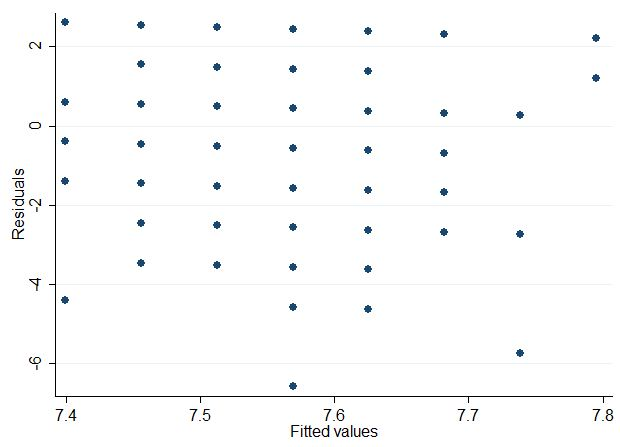
\includegraphics[width=1\textwidth]{./figures-and-tables/conc-linear-resid-vs-fitted.jpeg}};
    \end{tikzpicture}
    \label{fig:conc_rvfp}
\end{figure}

% M8: it's curvilinear! http://www.philender.com/courses/linearmodels/notes3/curve.html
% ref for great stat interpretation: http://people.umass.edu/biep640w/pdf/Stata%20Illustration%20simple%20and%20multiple%20linear%20regression.pdf
% ref: https://stats.idre.ucla.edu/other/mult-pkg/faq/general/faqhow-do-i-interpret-the-sign-of-the-quadratic-term-in-a-polynomial-regression/
% ref: heatmap https://fmwww.bc.edu/repec/dsug2019/germany19_jann.pdf
% ref: correlation table https://lost-stats.github.io/Presentation/heatmap_colored_correlation_matrix.html#stata
Model 8 captures this curvilinear relationship by expanding Model 7 with quadratic and cubic factors.
% Quadratic factors in this model represent marginal effects.
% Cubic effects capture marginal changes in the marginal effects.
The coefficients in this model are not significant, but the directions of effect are as expected.
In this model, the average total effect of the comparative conscientiousness gap on hireability is negative\footnote{
    Computed as:
    $-0.0018 = - 0.0524*0.0330 - 0.0465*0.0330^2 + 0.0380*0.0330^3$
}.
The average total effect for Model 8 as a whole is also negative\footnote{
    Computed as:
    $-0.0293 = -0.1444*0.1415 + 0.0340*0.1415^2 - 0.0194*0.1415^3 - 0.0803*0.0943 - 0.0112*0.0943^2 - 0.0023*0.0943^3 - 0.0524*0.0330 - 0.0465*0.0330^2 + 0.0380*0.0330^3$
}.
When the comparative gap in conscientiousness increases above the average of 0.33,
the linear effect is negative and the marginal effect is also negative,
but the marginal effect is becoming less negative as conscientiousness increases.

Models 7 and 8 provide a skill-level diagnostic in service of closing the demand gap for ACNG labor.
Alternative learning providers can implement body language communication training in their products,
or ACNG candidates can obtain additional training and credentials that target this skill a la cart.
% Improving body language communication skill is precisely diagnosed and not to be confused with generalized communication skill.
% Perceived skill gaps for emotional intelligence, verbal communication, and written communication are insignificant.
ACNG job candidates can offset perceived conscientiousness deficit by provisioning work history or results of a personality test.
External research indicates that psychological therapy and other interventions can boost conscientiousness in some cases\cite{kilduff_tasselli_landis_2018}.

\section{Conclusion}

% TODO: long paper food...talk about job candidate stigma mitigation techniques and hope for the ACNG
%       ACNG is not strictly dispreferred to the college grad, they just need to find a well-fitting employer
This study provides evidence that skill signals are an important factor of hireability and are unique for the ACNG.
Perceived skill gaps do a better job of explaining hireability than other widely recognized effects like industry and state effects.
Employer factors better explain candidate hireability than do the perceived skill gaps themselves.
Technical skill gaps explain less about hireability than soft skill gaps for ACNG job candidates.

The classic signaling model explanation for employer preference of college graduate labor over ACNG labor is that
the college degree provides a comparative signal of conscientiousness and conformity.
The present paper finds evidence that conscientiousness is an important comparative difference contributing to weak ACNG demand,
but conformity does not have such a general effect.
This paper finds that employers of different types have qualitatively different views about conformity.
Some employers demand conformity, but many demand nonconformity.

This paper provides evidence that some employers engage in conformity selection to avoid risk to the reputation, productivity, or value of a company.
Ironically, such employers fail to conform to normal behavior.
Respondents most often preferred to describe nonconformists as individuals who could just as easily be high performers as low performers.
An explanation from risk aversion is preferred because it explains low ACNG labor demand from an employer given either of the above responses.
Positive conformity selection is only able to explain the former case.

Risk aversion and conformity selection are both partially unconscious biases that lead to an inefficient organizational operation.
A practical recommendation is for organizations to implement bias controls concerning ACNG evaluation.
An example control would be to provide human resource procedures for formal evaluation of particular credentials relevant to specified job families.
These procedures provide immediate operational benefits regarding known credentials and job families.
These procedures should also be retained for ongoing application as new credentials are developed and encountered over time.
% Adjustments can be applied to new hires or during performance reviews for current employees.

Another action item is for educational institutions, policymakers, and the general public to invest further in correcting alternative education misinformation.
A survey on trade schooling taken in 2019 provides evidence on the role of this kind of misinformation\cite{arabia_2019}.
Only 27 percent of respondents correctly responded that lower debt is an advantage of enrolling in trade school relative to college.
Additionally, over 75 percent of respondents failed to notice that trade school graduates receive industry employment sooner
and receive specialized training when compared to a four-year college.
% The news that employers are generally favorable to alternative credentials should be shared far and wide.
% The current education system should be reformed to better inform students about non-college career entry.

Obtaining a college degree after obtaining some work experience will allow students to leverage employer tuition benefits.
Because ACNG hireability varies importantly by the particular employer, ACNG job candidates can reduce the risk of a lengthy job search by applying to many employers at the outset of the job search.
Social networking, online research into firm policy, and consulting with recruiters or other industry specialists are tactics to apprehend whether a particular employer is a likely member of the set that is favorable to ACNG labor.
% Government should emphasize job skills over the formal degree.
% Recent moves have begun such emphasis\cite{https://www.usatoday.com/story/news/politics/2020/06/26/trump-executive-order-stresses-skill-over-college-degree-hiring/3263074001/}

% Out of scope for this paper, but important:
% 1. aggregate social, legal, political, and economic movements (aggregate study is wanting, we know states, time, industry all matter)
% 2. applicant personal effects, and interviewer-applicant interaction effects
% despite those caveats, we can reasonably explain employer hireability their imagined candidate based on matching effects

The preferred model explains about one-third of hireability.
Perceived skill gaps and rulebreaker effects account for most of the explanatory power in the model.
There are several means of extending this research to provide improved explanatory power.
A longitudinal study would allow for causal analysis and improve forecasting of ACNG hireability in the future.
Other research has conducted some dynamic analysis of the same dependent variable with different regressors\cite{vandivier2020preliminary}.
Analysis that includes overqualification effects and heterogeneous nonlinear relations between skill gaps and hireability would improve estimates of hireability for a candidate of a particular skill profile.

% TODO: this paragraph not needed in short paper
This paper noted that large employers and the information technology industry have a peculiar susceptibility to alternative credentials, so recent changes implemented by Google may indicate future trends.
Google has not required a college degree since before 2013\cite{bryant2013head}.
Laszlo Bock, then Senior Vice President of People Operations at Google, stated the following in 2013:
"After two or three years, your ability to perform at Google is completely unrelated to how you performed when you were in school, because the skills you required in college are very different."
In 2020, Google added three new certificate programs to an existing set and declared that all of its certificates are equivalent to an undergraduate degree for their hiring purposes\cite{hess_2020}.

If perceived skill represents actual skill, then this study provides evidence that employers should be more willing to hire an ACNG.
At the same time, this paper provides evidence that perceived and actual skill levels sometimes do not align.
For example, the average recent college graduate in the sample has more perceived technical skills than the average ACNG.
The perceived technical deficiency among ACNG labor is surprising because last-mile training, a kind of alternative education, has been specifically recommended in popular literature to remedy the technical skill gaps among recent college graduates.
Further study of the differences between perceived and actual skills is encouraged.

Employers seem to be favorable to individuals with alternative credentials.
In many cases, employer-perceived skill gaps are not statistically different when comparing recent college graduates with ACNG candidates.
Instead of looking to actual or perceived skill differences,
the college degree's social status may be better explained by public ignorance about appropriate alternative programs,
a lack of appropriate programs for certain occupations, and government policy that gives preference to accredited education.

% Notice that the alternatively credentialed individual doesn't need the average employer to value him or her.
% He or she simply needs some significant chance of being hired, and that certainly exists.
% Moreover, the average employer is already favorable to alternative credentials.
% As more alternatively credentialed individuals are highered and promoted through society,
% there is reason to think the number of opportunities afforded to alternatively educated individuals may grow.
% The problem doesn't seem to be about whether alternative credentials work, but whether they exist in a given industrial context,
% and whether an individual would like to pay the college premium for better hireability when both options are feasible.

\bibliography{./BibFile}

\end{document}
